\section{Optimization}
To maximize the cumulative discounted profit in a framework of NaaA,
it is important to balance the two contradicting criteria: revenue $r_{it}$ and cost $c_{it}$.

%TODO: 否定的な結論。何が問題か、E

%\begin{thm}\label{thm:optimal-bidding-simple}
%	The Nash equivalent of the game $(r_{ijt})$ is $0$.
%\end{thm}
%ただちに、次の系が�E立する、E
%\begin{coro}\label{coro:optimal-bidding-simple}
%NaaA では、外的環墁E��ら報酬を受け取らなぁE��ューロンはすべて NOOP になる、E
%\end{coro}

To achieve that, we use the mechanism design.
We introduce mechanism design because, unlike several existing studies \citep{sukhbaatar2016learning}, NaaA assumes that all agents are not cooperative but selfish.
%(TODO: こ�Eあたり�E斁E��は要検訁E
If we naively optimize the optimization problem of NaaA, then we obtain the trivial solution that the internal rewards will converge to 0, and that all the units become NOOP.
Therefore, the multi-agent system should select the action with no information. It is equivalent to taking an action randomly.
For that reason, the external reward $R_t^{\mathrm ex}$ shrinks markedly.

%これは、ナチE��ュ坁E��がパレート最適と一致しなぁE��レート劣位な状況が発生する、E

\subsection{Envy-free Auction}
To achieve Pareto optimality, we borrow the idea from the digital goods auction.
The auction theory belongs to mechanism design. It is intended to unveil the true price of goods.
Digital goods auction is one mechanism from auction theory.
It is target to copyable goods without cost, such as digital books and music.

Although several variations of digital goods auctions exist,
we use an envy-free auction \citep{guruswami2005profit} because it requires a simple assumption: the same goods have one price simultaneously.
In NaaA, it can be represented as the following assumption:
\begin{enumerate}
\renewcommand{\labelenumi}{N\arabic{enumi}:}
\setcounter{enumi}{4}
\item (Law of one price)
	If $\rho_{j_1,i,t}, \rho_{j_2,i,t} > 0$, then $\rho_{j_1,i,t} = \rho_{j_2,i,t}$.
\end{enumerate}
Therefore, $\unit$ has an intrinsic price at the same timing $t$.
We denote the price as $q_{it}$.

\begin{figure*}[t]
\centering
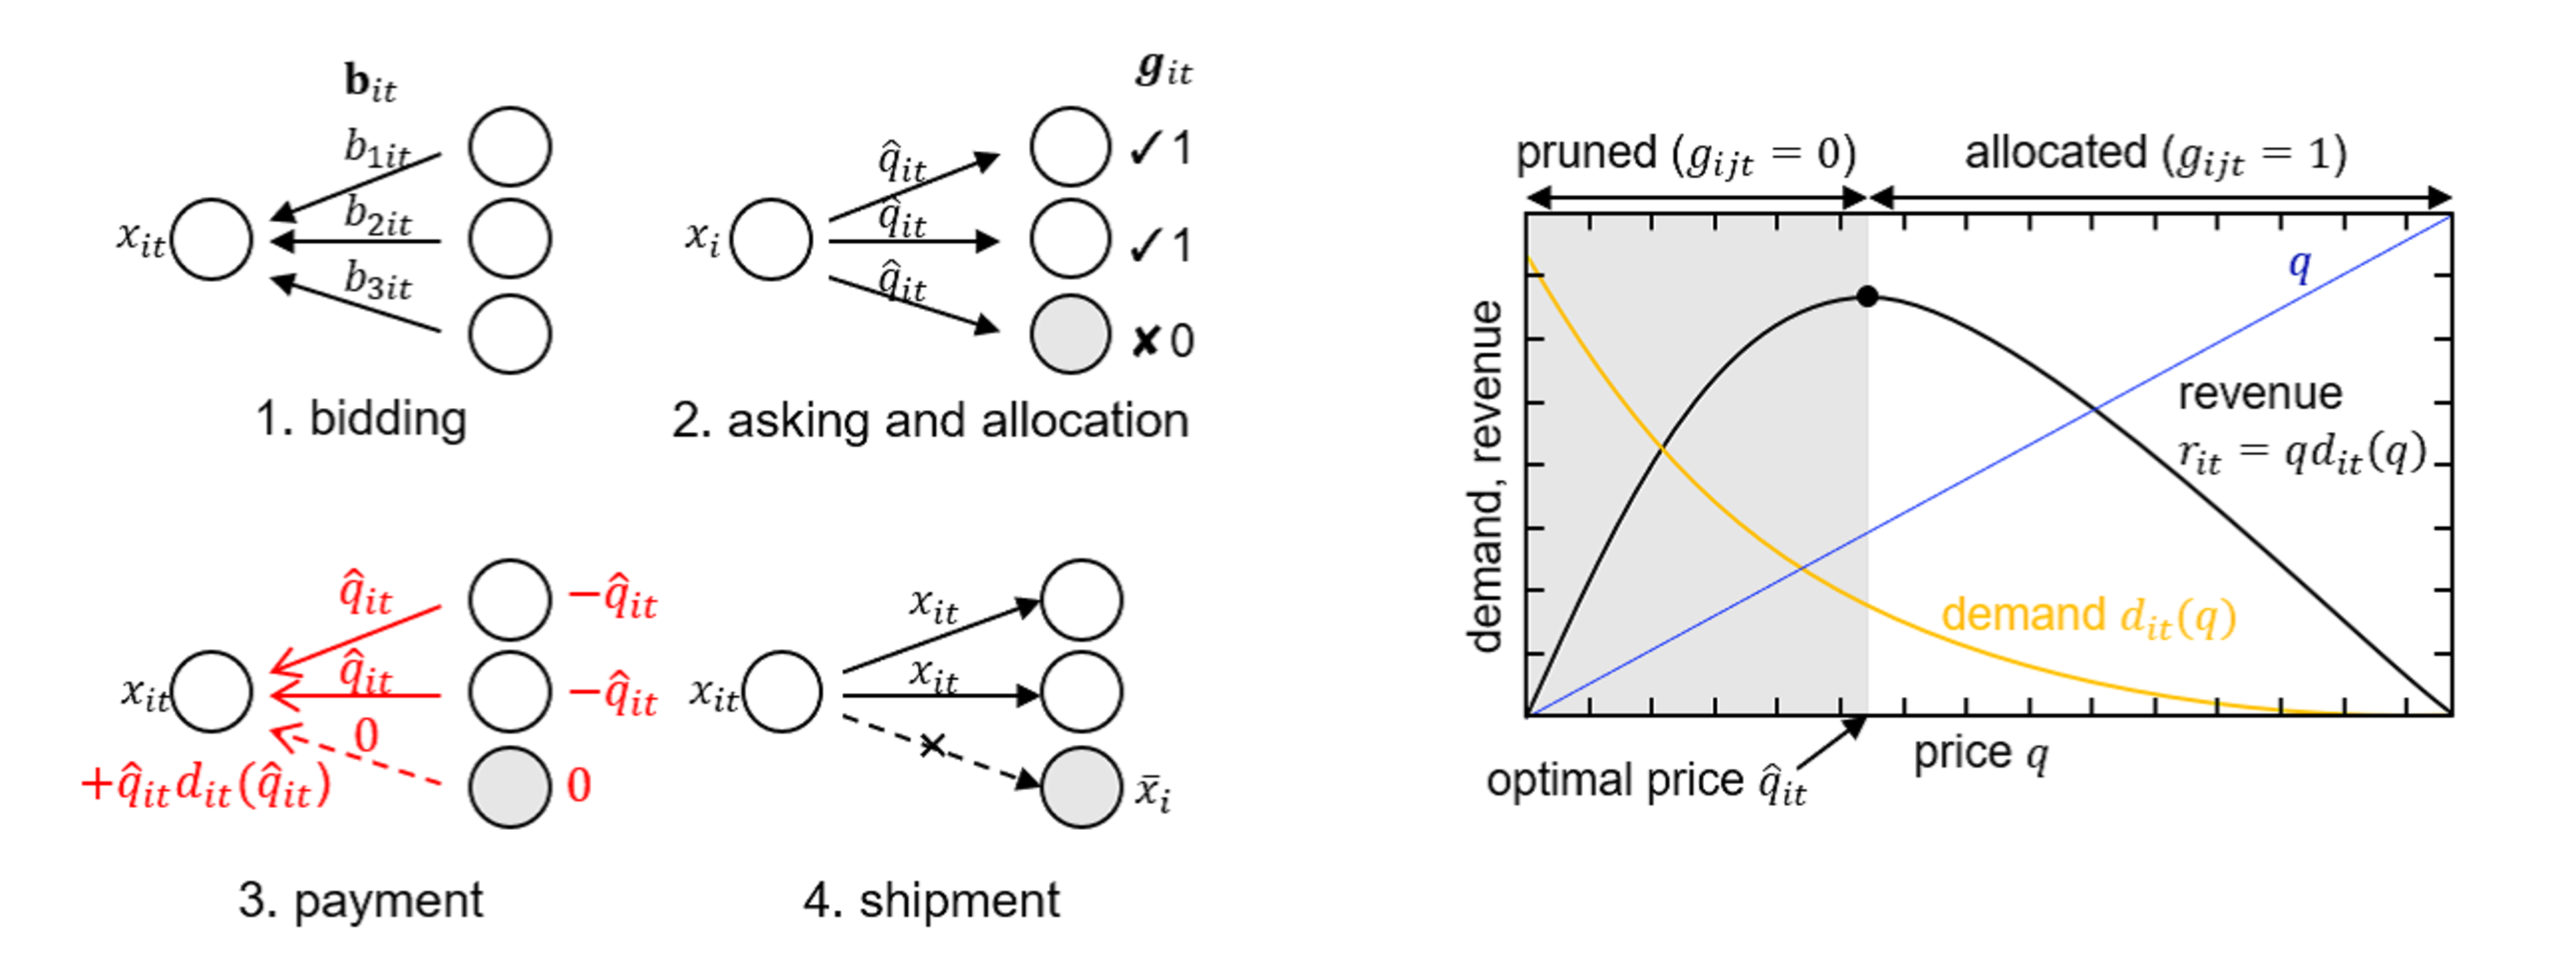
\includegraphics[width=\linewidth]{img/double.eps}
\caption{
\textbf{Left}: The process of trade in an envy-free auction.
\textbf{Right}: A price determination curve for a unit. Revenue of a unit is a product of monotonically decreasing demand and price. The price maximizing the revenue is the optimal price.
}
\label{fig:double}
\end{figure*}

% TODO 割当�E話
We present the envy-free auction process at the left of Figure \ref{fig:double}.
It shows the negotiation process between one unit in sending activation and a group of units that buy the activation.
The negotiation performed per time step in RL.
We name the unit in sending activation as a seller, and units in buying activation as buyers.
First, the buyer bids the unit in bidding price $b_{jit}$ (\textbf{1}).
Next, the seller decides the optimal price $\opt{q}_{it}$, and performs allocation (\textbf{2}).
After allocation, the buyers perform payment as $\rho_{jit} = g_{jit} \opt{q}_{it}$ (\textbf{3}).
The seller only sends activation $x_i$ to the allocated buyers (\textbf{4}).
A buyer which cannot receive the activation approximates $x_i$ with $\Expect{\pi}{x_i}$.

In the following, we discuss revenue, cost, and value functions based on Eq:(\ref{eq:V}).

%以下では、Envy-free auction における収盁E$r_{it}$ とコスチE$c_{it}$ の最適化につぁE��刁E��て説明を行う、E

%こ�E過程�E、本めE��楽などの、褁E��可能財、digital goods を対象にしたオークション琁E��Edigital goods auction において、E
%envy-free auction として知られてぁE��、E
%後で示すよぁE��、このシンプルな前提のみでジレンマ�E問題が解決する、E
%NaaA による取引�E流れを図\ref{fig:double}に示す、E

%========================================
% 収益
%========================================

\textbf{Revenue}:
The revenue of a unit is given as
\begin{flalign}
	r_{it}  &= \sum_{j \in N^\mathrm{out}_i} g(b_{jit}, q_{it}) q_{it} + R^\mathrm{ex}_i  = q_{it} \sum_{j \in N^\mathrm{out}_i} g(b_{jit}, q_{it})  + R^\mathrm{ex}_i \notag \\
		&= q_i d_{it}(q_t) + R^\mathrm{ex}_i,
\end{flalign}
where $g(\cdot, \cdot)$ is allocation. It is defined using a step function $H(\cdot)$ as $g(b,q)=H(b - q)$.
$d_{it}(q_{it})$ is a count of units for which the bidding price for $q_{it}$ is greater than or equal to $q_{it}$, designated as demand.
$q_{it}$ maximizing the equation is designated as the optimal price. It is denoted as $ \opt{q}_{it} $.
Because the second term in the equation is independent of $q_t$, the optimal price $\opt{q}_{it}$ is given as
\begin{flalign}
	\opt{q}_{it}  = \argmax_{q \in [0, \infty)} q d_{it}(q).
\end{flalign}
We present the curve of $q_{it}$ on the right side of Figure \ref{fig:double}.

%========================================
% コスチE
%========================================
\textbf{Cost}:
The cost is an internal reward that the unit should pay to other units.
It is represented as shown below.
\begin{flalign}
	c_{it} = \sum_{j \in N^\mathrm{in} } g(b_{ijt}, q_j) q_j
\end{flalign}
Although $c_{it}$ itself is minimized when $b_{ijt} = 0$,
this represents a tradeoff with the following value function.

\textbf{Value Function}:
%Value of the value function $V(s_{i,t+1})$ depends on $s_{i,t+1}$.
%As we already defined, the internal environment of $v_i$ is a set of connected units,
%and the output of units affect to evaluation from the units, namely, weight of edges.
%As the learning rule of a typical artificial neural network obeys to law of Hebb, 
%the reward becomes lower because weight of unit which do not contribute
%the accuracy of output becomes lower.
Activation $x_i$ depends on input from the units in $N_i^{\mathrm in}$. It affects the bidding price from units in $N_i^{\mathrm out}$.
If we minimize $b_{ijt}$ and let $b_{ijt} = 0$, then the purchase of activation fails, and the reward the unit can obtain from the units to which 
the unit connects becomes lower in the future.

Then, we designate the allocation as $\vect{g}_{it} = (g_{i1t}, \dots, g_{iNt})^\T$, 
and consider effects for value functions in the cases when a unit succeeds in purchasing $v_j$ or not.
The value function can be written as the equation using a state-value function $Q(s_{i,t+1}, \vect{g}_{i,t+1})$.
\begin{flalign}
	V_i^{\pi_i}(s_{it}) 
	&= Q_i^{\pi_i}(s_{it}, \vect{g}_{it}) \notag \\
	&= \sum_{j \in \followees} g_{ijt} (Q_i^{\pi_i} (s_{it}, \vect{e}_j) - Q_i^{\pi_i}(s_{it}, \vect{0})) + Q_i^{\pi_i}(s_{it}, \vect{0}) \notag \\
	&= \sum_{j \in \followees} g_{ijt} o_{ijt} + Q_i^{\pi_i}(s_{it}, \vect{0}) \notag \\
	&= \vect{g}_{it}^\T \vect{o}_{it} + Q_i^{\pi_i}(s_{it}, \vect{0})
\end{flalign}

We designate $o_{ijt} = Q_i^{\pi_i} (s_{it}, \vect{e}_j) - Q_i^{\pi_i}(s_{it}, \vect{0})$ as the {\em counterfactual return}, 
which is equivalent to the cumulative discount value of counterfactual reward \citep{agogino2006quicr}.
That is, the cost the unit will pay is $\opt{q}_{it}$ in success of purchasing data, and $o_{it}$ otherwise.

Therefore, the optimization problem is presented below.
\begin{flalign}
	\max_{\vect{b}, q} \Expect{\hat{\vect{q}}_t}{ V_i^{\pi_i}(s_{it}) } = 
		\max_q q d_{it}(q) - 
		\min_{\vect{b}} \Expect{\hat{\vect{q}}_t}{\vect{g}_{it}(\vect{b})^\T( \hat{\vect{q}}_t - \gamma \vect{o}_{i,t+1}  )} + \const.
\end{flalign}
We take the expectation $\Expect{\hat{\vect{q}}_t}{\cdot}$ 
because the asked price $\hat{\vect{q}}_t$ is unknown for $v_i$, except for $\hat{q}_{it}$, and $g_{iit} = 0$.

Then, what is bidding price $b_{it}$ to maximize return?
The following theorem holds.

\begin{thm}\label{thm:optimal-bidding}
	(Truthfulness) the optimal bidding price for maximizing return is $\opt{\vect{b}}_{it} = \vect{o}_{it}$.
\end{thm}
See the Appendix for the proof.

That is, the unit should only consider its counterfactual return (!).
Consequently, in the mechanism of NaaA, the unit obeys as if performing valuation to the other units, 
and declares the value truthfully.

Then, the following corollary holds:
\begin{coro}\label{coro:optimal-bidding}
	The Nash equilibrium of an envy-free auction $(\vect{b}_{it}, q_{it})$ is $(\vect{o}_{it}, \argmax_{q} q d_{it}(q))$.
\end{coro}


